\chapter{Context update}

The context update network has to approximate Equation~TODO which, as a reminder, is restated here:
\begin{equation}
    \ctx_i = \rho_i \ctx_{i-1} + \tcmbeta \ctxin_i\,\text{.} \label{eqn:ctx-update}
\end{equation}
Different methods of approximating this equation can be thought of and in the following I will describe four methods of which only one was successful in matching the data.
Even though most of these methods have been unsuccessful it is instructive to see why these methods failed to match the data as this demonstrates which features of the mathematical TCM formulation are relevant and which are non-relevant side-effects of a particular formulation.

\section{Boundend integrator}
Equation~\ref{eqn:ctx-update} assumes discrete steps, but for a neural implementation a continuous formulation is more natural and given by
\begin{equation}
    \od{\ctx}{t} = (\bar{\rho} - 1) \ctx + \bar{\tcmbeta} \ctxin\,\text{.}
\end{equation}
This equation is easily implemented with a neural integrator for a constant $\bar{\rho}$ and $\bar{\tcmbeta}$.
However, there is no limit on the integration of $\ctxin$ anymore.
To add at most $\tcmbeta \ctxin$ to the context $\ctx$, we can gate the input to the integrator and add a network computing the dot product between $\ctx$ and $\ctxin$.
After thresholding it at $\tcmbeta$, it can be used to suppress the input by inhibiting the gate (see \cref{fig:ctx-bounded-integrator}).
Furthermore, $\bar{\rho}$ needs to be adjusted to keep the unit length of $\ctx$.
To do so, we can project $\ctx$ to another population $\ctx_{\downarrow}$ which projects back to the integrator with a transform of $\gamma = -0.1$.
Picking a $\gamma$ closer to zero will allow the $\vc c$ vector exceed unit length by a larger amount while the integrator receives input and will increase the time required to settle back to unit length, whereas a large magnitude of $\gamma$ can lead to oscillatory behaviour.
The $\ctx_{\downarrow}$ population needs to be controlled to only provide the inhibitory input to the integrator as long as $\norm{\ctx} > 1$.
This is achieved by decoding the length of $\vc c$ from the integrator and thresholding it at $1$.
As long as the threshold is not exceeded, $\ctx_{\downarrow}$ will be inhibited.
\begin{figure}
    \centering
    \begin{tikzpicture}[nef]
        \graph {
            in/\ctxin [ext] -!- {
                gate/ [ea] -> ["$\bar{\tcmbeta}$"] integrator/\ctx [ea] -> out/ [ext],
                threshold/ [rect] -!- downscale/$\ctx_{\downarrow}$ [ea] -!- length/ [rect],
                dot [net]
            },
            in -> gate,
            in -> dot -> threshold -> [inhibit, "$\Heavi(x - \bar{\tcmbeta})$" {rotate=90}] gate,
            integrator -> dot,
            integrator -> [recurrent, "$\bar{\rho}$" above] integrator,
            integrator -> [bend right] downscale -> [bend right, "$\gamma$" {below, rotate=270}] integrator,
            integrator -> ["$1 - \norm{\ctx}$" {anchor=south west}] length -> [inhibit] downscale
        };
    \end{tikzpicture}
    \caption{Bounded integrator network.}\label{fig:ctx-bounded-integrator}
\end{figure}

As a basic test I fed the network with nearly orthogonal context vectors $\ctxin$ at a rate of one vector per second and record the represented context $\ctx$.
The context drift parameter was set to $\tcmbeta = 0.6$.
I present three metrics to evaluate the performance of the network.
First, the norm of the context vector $\norm{ctx}$ which should stay close to one.
Second the effective context drift $\tcmbeta'$ which is the similarity of the represented context $\ctx$ and the new context vector $\ctxin$.
For orthogonal $\ctxin$ vectors, the effective context drift $\tcmbeta'$ should rise to $\tcmbeta$, but note that for non orthogonal vectors an effective context drift of more than $\tcmbeta$ is expected.
In this latter case the input context vectors $\ctxin$ are still supposed to be added with a strength of $\tcmbeta$, but because the context $\ctx$ will already be similar to $\ctxin$, the updated context vectors should have a higher similarity to $\ctxin$ than $\tcmbeta$.
Third and most importantly, it is useful to look at the decay of the context similarity over time for each updated context vector which is given by $\ctx_i \cdot \ctx(\Delta t)$ with $\Delta t = t - i \cdot \SI{1}{\second}$.
The $i$-th context vector in this context is defined as $\ctx_i = \langle \ctx(t) \rangle_{t \in \interval[open right]{i + \SI{0.7}{\second}}{i + \SI{1}{\second}}}$.

\Cref{fig:bounded-integrator-orthogonal} shows these metrics for the bounded integrator network. With the orthogonal input contexts it seems to be working properly.
The norm of the context vectors stays at one, the effective $\tcmbeta$ rises to $\tcmbeta$ for each new input vector, and the context similarity decay is roughly what is expected despite a few traces decaying too quickly.
However, the network fails, if the input context vectors are not orthogonal, but have a similarity of about $0.6$ (\cref{fig:bounded-integrator}).
In this case, the context similarity does not decay nearly as quickly as it should.
This can be attributed to stopping the updating once the effective $\tcmbeta$ reaches $\tcmbeta$ even though in the case of similar input vectors this is not sufficient.
\begin{figure}
    \centering
    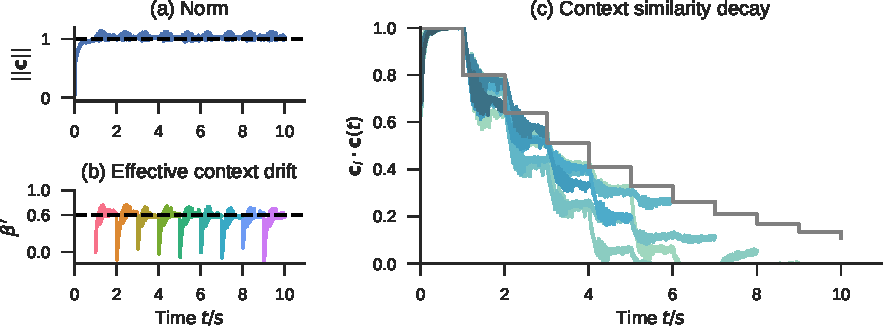
\includegraphics{context-analysis/bounded-integrator-orthogonal}
    \caption{
        Properties of the context vectors produced by the bounded integrator network with orthogonal input context vectors.
        (a) Norm of the context vector over time.
        (b) Effective context drift $\tcmbeta'$ for each input context vector. The dashed line indicates the value of the context drift parameter $\tcmbeta$.
        (c) Blue lines: Context similarity decay $\ctx_i \cdot \ctx(\Delta t)$ for each context vector $\ctx_i$. Gray line: Expected context similarity decay.
    }\label{fig:bounded-integrator-orthogonal}
\end{figure}
\begin{figure}
    \centering
    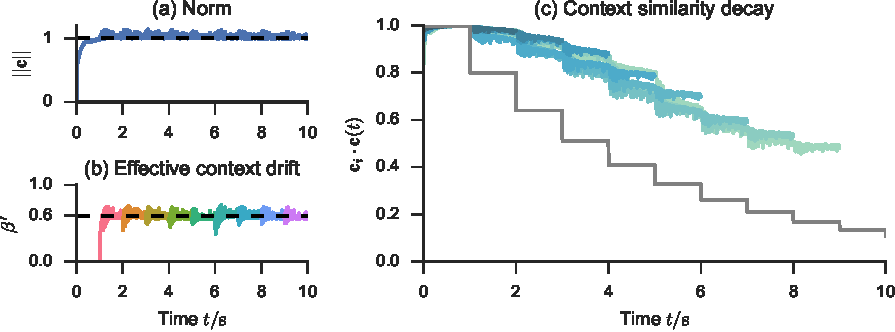
\includegraphics{context-analysis/bounded-integrator}
    \caption{
        Properties of the context vectors produced by the bounded integrator network with a similarity of about $0.6$ between successive input context vectors.
        (a) Norm of the context vector over time.
        (b) Effective context drift $\tcmbeta'$ for each input context vector. The dashed line indicates the value of the context drift parameter $\tcmbeta$. The effective drift is supposed to be higher for non-orthogonal inputs.
        (c) Blue lines: Context similarity decay $\ctx_i \cdot \ctx(\Delta t)$ for each context vector $\ctx_i$. Gray line: Expected context similarity decay.
    }\label{fig:bounded-integrator}
\end{figure}

\section{Alternating memory buffers}
With a single integrator we have to rely on the dot product between the input context vector and current context as a measure of $\tcmbeta$.
To circumvent this we need to use to gated memory populations that are updated in alternating fashion.
Then the output of the old context and input vector can be combined according to $\rho \ctx + \tcmbeta \ctxin$ and fed into to the memory buffer for the current context (\cref{fig:ctx-amb}).
The completion of that memory update can be detected by the dot product of the updated context and the current context crossing a threshold of 1.
\begin{figure}
    \centering
    \begin{tikzpicture}[nef, x=2cm, y=2cm]
        \graph [no placement] {
            in/\ctxin [ext, at={(0,0)}] -> ["$\tcmbeta$"] new/ [pnode, at={(1,0)}] -> cgate/ [ea, at={(2, 1)}] -> current/\ctx [ea, at={(3, 1)}] -> oldgate/ [ea, at={(3, -1)}] -> old/$\ctx'$ [ea, at={(2, -1)}] -> ["$\rho$"] new,
            current -> [bend right, "$-1$"] cgate,
            new -> [out=0, in=225] dot [net, at={(4, 1)}], current -> dot [net],
            dot -> rectification/ [rect, at={(4.5, 0.5)}] -> ["$\Heavi(x)$" anchor=west] heavi/ [pnode, at={(4.5, -0.5)}] -> [inhibit, bend left] cgate,
            heavi -> [inhibit] invert/ [ens, at={(4, -1)}] -> [inhibit] oldgate,
            bias/1 [ext, at={(4.5, -1)}] -> invert,
            old -> [bend right, "$-1$" below] oldgate
        };
    \end{tikzpicture}
    \caption{Context network with alternating memory buffers.}\label{fig:ctx-amb}
\end{figure}

Unfortunately, this still does not work for similar input context vectors (\cref{fig:amb}).
In that case the dot product of the updated context and current context will already be quite high and the updated context is not completely loaded into the current memory buffer.
Again the context drift and similarity decay will be too slow.
\begin{figure}
    \centering
    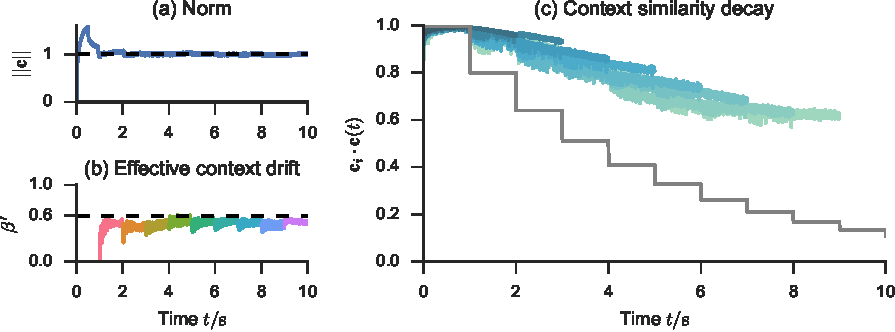
\includegraphics{context-analysis/amb}
    \caption{
        Properties of the context vectors produced by the update of two alternating memory buffers with a similarity of about $0.6$ between successive input context vectors.
        (a) Norm of the context vector over time.
        (b) Effective context drift $\tcmbeta'$ for each input context vector. The dashed line indicates the value of the context drift parameter $\tcmbeta$. The effective drift is supposed to be higher for non-orthogonal inputs.
        (c) Blue lines: Context similarity decay $\ctx_i \cdot \ctx(\Delta t)$ for each context vector $\ctx_i$. Gray line: Expected context similarity decay.
    }\label{fig:amb}
\end{figure}


\section{Externally controlled alternating memory buffers}
All approaches to determine required context updates based on vector similarity will fail because the similarity of $\ctxin_i$ and $\ctx_{i-1}$ is not known beforehand and can vary widely depending on what contexts are recalled.
Thus, for a properly working context update in the TCM model, the update process has to be controlled by an external control signal (\cref{fig:ctx-ext-amb}) (TODO reference other chapter).
If we take the alternating memory buffer network, but control it externally, it works for both orthogonal and similar input vectors (\crefrange{fig:ctx-ext-amb}{fig:ext-amb}).
\begin{figure}
    \centering
    \begin{tikzpicture}[nef, x=2cm, y=2cm]
        \graph [no placement] {
            in/\ctxin [ext, at={(0,0.5)}] -> ["$\tcmbeta$"] new/ [pnode, at={(1,0.5)}] -> cgate/ [ea, at={(2, 1)}] -> current/\ctx [ea, at={(3,1)}] -> oldgate/ [ea, at={(3, -1)}] -> old/$\ctx'$ [ea, at={(2, -1)}] -> ["$\rho$" {very near start, below}] new,
            current -> [bend right, "$-1$"] cgate,
            ctrl [ext, at={(0,-.5)}] -> pctrl/ [pnode, at={(1,-.5)}] -> [inhibit] cgate,
            pctrl -> ["$-1$" near end] invert/ [pnode, at={(2.5, -0.5)}] -> [inhibit] oldgate,
            bias/1 [ext, at={(2.5, 0)}] -> invert,
            old -> [bend right, "$-1$" below] oldgate
        };
    \end{tikzpicture}
    \caption{Context network of externally controlled alternating memory buffers. The control signal \pop{ctrl} is externally provided and switches which memory buffer is updated.}\label{fig:ctx-ext-amb}
\end{figure}
\begin{figure}
    \centering
    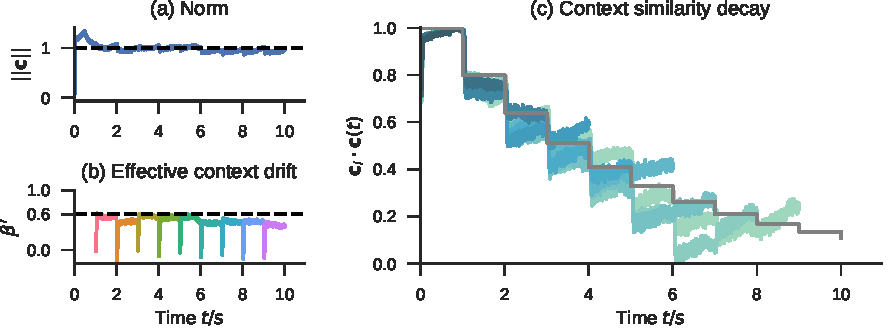
\includegraphics{context-analysis/ext-amb-orthogonal}
    \caption{
        Properties of the context vectors produced by the externally controlled alternating memory buffers with nearly orthogonal input context vectors.
        (a) Norm of the context vector over time.
        (b) Effective context drift $\tcmbeta'$ for each input context vector. The dashed line indicates the value of the context drift parameter $\tcmbeta$.
        (c) Blue lines: Context similarity decay $\ctx_i \cdot \ctx(\Delta t)$ for each context vector $\ctx_i$. Gray line: Expected context similarity decay.
    }\label{fig:ext-amb-orthogonal}
\end{figure}
\begin{figure}
    \centering
    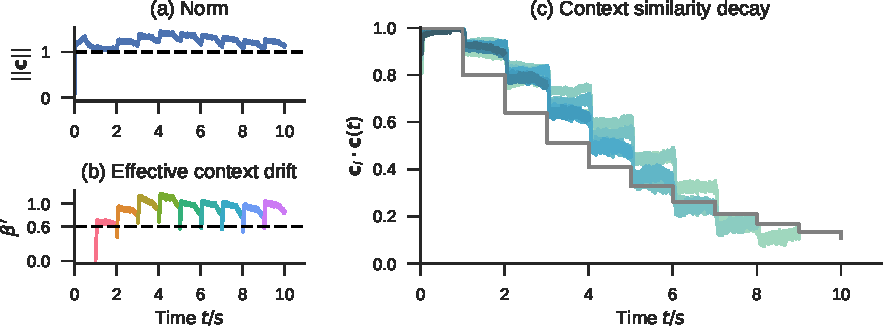
\includegraphics{context-analysis/ext-amb}
    \caption{
        Properties of the context vectors produced by the externally controlled alternating memory buffers with a similarity of about $0.6$ between successive input context vectors.
        (a) Norm of the context vector over time.
        (b) Effective context drift $\tcmbeta'$ for each input context vector. The dashed line indicates the value of the context drift parameter $\tcmbeta$. The effective drift is supposed to be higher for non-orthogonal inputs.
        (c) Blue lines: Context similarity decay $\ctx_i \cdot \ctx(\Delta t)$ for each context vector $\ctx_i$. Gray line: Expected context similarity decay.
    }\label{fig:ext-amb}
\end{figure}

This leads to a number of predictions.
First, the update of the context signal is not directly regulated by the input, but externally controlled.
Second, there are neural populations that will start representing the current context in succession.
